% !TEX root = ../Thesis.tex
\chapter{Results}

\section{Fork-Write Benchmark}

First, the simple fork-write benchmark used in the Trap-Driven Simulation evaluation is used as a basic demonstration of the superpage overlay framework. This is done with 2MB of memory allocated as a superpage, and varying amounts of writing. The superpage is split when COW occurs to minimize the amount of memory copied. Figure \ref{fig:forkwrite} shows that in that workload, overlays yield a constant reduction of about 512 4KB TLB misses. Without overlays, the child process causes about 512 TLB misses looping through the 2MB of memory, and an additional TLB miss for each page it writes to because of COW. With overlays, the page stays as a superpage, so there is only one TLB miss per page overlaid-on-write.
\begin{figure}
    \centering
    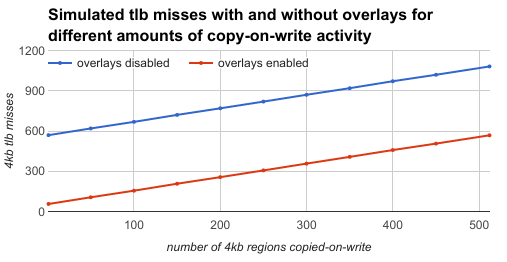
\includegraphics[width=5in]{Figures/Graph1}
    \caption{TLB misses with and without overlays on the fork-write benchmark}
    \label{fig:forkwrite}
\end{figure}

If the superpage were not split for COW, there would be only two 2MB TLB misses without overlays and very few 4KB TLB misses, since the only interesting memory is the original superpage and its copy. Of course, in this case overlays cause more TLB misses but fewer pages copied unless every page is written to.

\section{Memory Checkpointing Benchmark}

This is the more interesting application to analyze. The default TLB parameters (4 way associative with 128 entries) are used, and checkpoints are taken every 1 second for 10 seconds. A fixed 10 million read/write iterations are carried out. First, the write probability is varied while keeping the default locality factor of $0.6$. TLB misses (Figure \ref{fig:write_prob_misses}) and the number of pages copied-on-write during the checkpoints (Figure \ref{fig:write_prob_copied}) are measured for the three types of COW: splitting superpages, retaining superpages, an overlay-on-write. Note that overlay-on-write copies the exact same number of pages as COW with splitting, since both simply copy each small page that is written to.
\begin{figure}
    \centering
    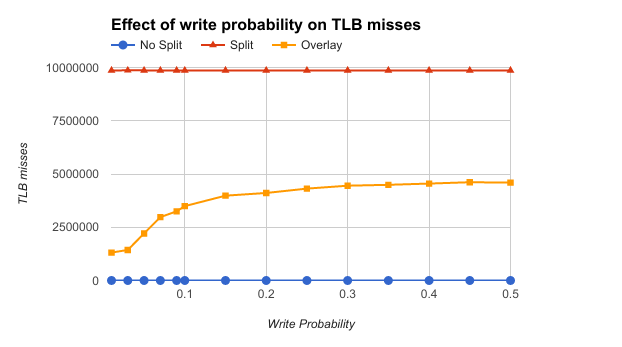
\includegraphics[width=6in]{Figures/write_prob_tlb}
    \caption{Write probability vs. TLB misses}
    \label{fig:write_prob_misses}
\end{figure}
\begin{figure}
    \centering
    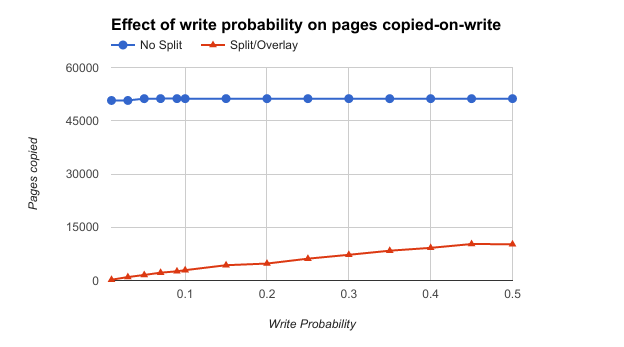
\includegraphics[width=6in]{Figures/write_prob_copied}
    \caption{Write probability vs. pages copied}
    \label{fig:write_prob_copied}
\end{figure}

Next, the same measurements are taken with a fixed write probability of $0.1$ while the locality factor varies (Figures \ref{fig:locality_misses} and \ref{fig:locality_copied}).
\begin{figure}
    \centering
    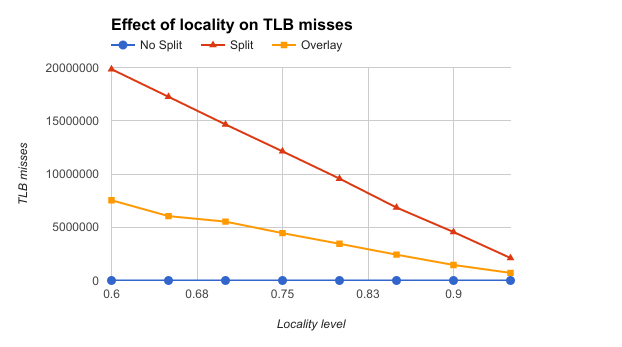
\includegraphics[width=6in]{Figures/locality_tlb}
    \caption{Locality vs. TLB misses}
    \label{fig:locality_misses}
\end{figure}
\begin{figure}
    \centering
    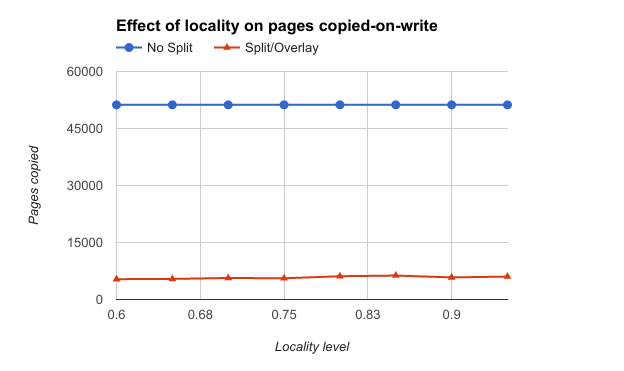
\includegraphics[width=6in]{Figures/locality_copied}
    \caption{Locality vs. pages copied}
    \label{fig:locality_copied}
\end{figure}

\subsection{Discussion}

This data clearly demonstrates the potential benefits of using superpage overlays.

\subsection{TLB misses}
The no-split case has a very small and consistent number of TLB misses, since the entire address space of the workload fits in the TLB when it is all in superpages. The split case, in contrast, produces a substantial number of TLB misses that directly depends on locality. That is simply because near-consecutive accesses to the same page will not cause TLB misses while every other access is likely to miss due to the large number of small pages. Even with a low write probability, the superpages are soon all split.

Overlays nicely split the difference between the split and no-split case. The TLB misses are related to locality in the same was as in the split case, and overlays benefit from a lower write probability because fewer overlays are created. Because of the overlay switching mechanism, the number of overlays should be bounded at half of the superpage, which means that there will be at most half as many small pages in the overlay case as in the split case. This is exactly what Figure \ref{fig:write_prob_misses} demonstrates.

\subsection{Data Copied}
For the number of pages copied, overlays simply give the same benefit that superpage splitting does. Like TLB misses, this metric benefits from low write probability, since more writes simply means more copies. The no-split case copies essentially the entire address space on every checkpoint, because even with high locality after 10 million iteration every superpage is likely to be touched.

\subsection{Overall Benefits}
As predicted, the superpage overlay system grants some of the TLB benefits of superpages while suffering none of the flexibility loss compared to small pages, as measured by the amount of memory affected by COW.

It is difficult to compare the TLB miss and page copy statistics directly because the cost of each of those is dependent on hardware specifics and overall cache behavior. However, we can get a general idea of the overall benefits of overlays by examining a simple hypothetical system. We estimate the cost of a TLB miss as roughly $5ns$ for a modern system \cite{Gorman}, and the time to copy a $4KB$ page as $100ns$ (write speed of 40GB/s). Then, we consider the data at locality $0.6$ and write probability $0.1$. From these numbers it is clear that TLB misses will dominate, since their numbers differ by up to 5 orders of magnitude between the no-split and split cases. So, the split case has $0.095s$ more overhead than the non-split case, while overlays only have $0.033s$ more. Both the split and overlay cases have only $10.4\%$ of the memory usage overhead that the no-split case exhibits; fewer page copies means less wasted memory.

This benchmark deals with a memory space that starts off entirely in superpages. If there was some nearly-aligned memory that never would be merged into a superpage without overlays, then the overlay case could easily perform better than the no-split case due to better superpage utilization. Also, if there were enough superpages to fill the 2MB TLB, the miss rates would be more similar and the cost of a page copy more significant. Finally, and most importantly, each page copy also uses up 4KB of memory in addition to taking time. Many systems operate under significant memory pressure and care more about reducing memory duplication than temporal overhead.

This data shows that if memory overhead is more, or even similarly, important compared to time overhead, superpage overlays are strictly better than splitting superpages and is likely to be preferable to using COW without splitting superpages.
